\documentclass[crop, tikz]{standalone}
\usepackage[utf8]{inputenc}
\usepackage[english, serbianc]{babel}
\usepackage{tikz}
\usepackage{amsmath}
\usepackage{bm}
\usepackage{amsthm}
\usepackage{amssymb}
\usetikzlibrary{calc}
\usetikzlibrary{calc, arrows.meta, positioning, backgrounds}
\usetikzlibrary{perspective}

\begin{document}
    \begin{tikzpicture}
        \node[anchor=south west,inner sep=0] (image) at (0, 0) {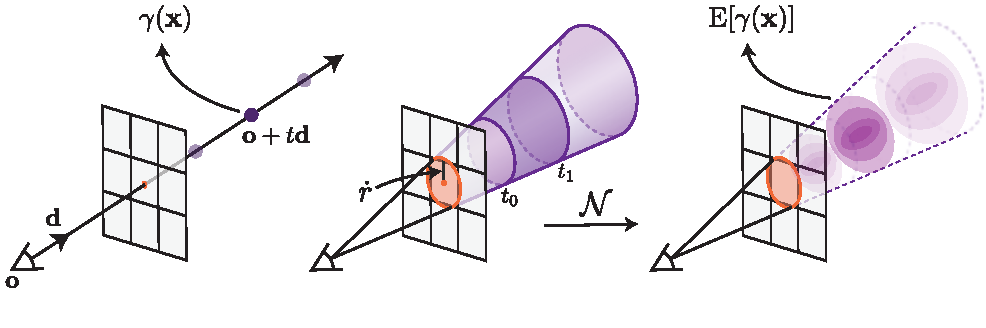
\includegraphics[width=\textwidth]{img/nerf_vs_mipnerf.pdf}};
        \begin{scope}[x={(image.south east)},y={(image.north west)}]
            \node[font=\small] at (0.2, 0) {NeRF};
            \node[font=\small] at (0.6, 0) {mip-NeRF};
            \fill[white] (0.352, 0.36) rectangle (0.377, 0.5);
            \node at (0.365, 0.43) {$R$};
            \fill[white] (0.7, 0.88) rectangle (0.83, 0.99);
            \node at (0.765, 0.945) {$\mathbb{E}(\gamma(\mathbf{x}))$};
        \end{scope}
    \end{tikzpicture}
\end{document}